\chapter{Sistema}

Cuando se realiza un reconocimiento facial podemos identificar una lista de pasos a seguir, los cuales forman el siguiente esquema:\\

\begin{figure}[H]
    \centering
    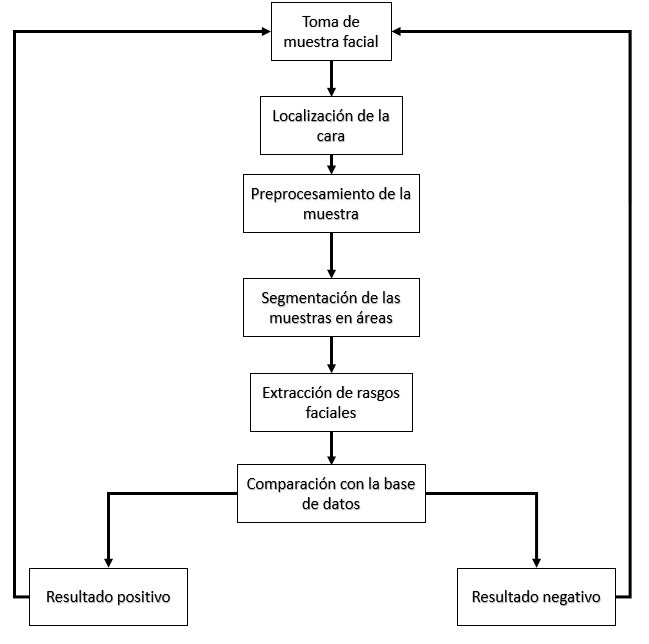
\includegraphics[width=0.85\textwidth]{Sistema.png}
    \caption{Pasos del sistema}
\end{figure}

Donde la localización de la cara consiste en la eliminación de información innecesaria que posea la muestra y el preprocesamiento consiste en mejorar la muestra obtenida.\\
Después realizamos una segmentación de lo que queda de la muestra para poder empezar a realizar el análisis de los rasgos faciales anteriormente mencionados. Una vez obtenidos se realiza una comparación con los datos biométricos de la base de datos y se obtiene un resultado. Independientemente del resultado, volveremos a realizar todo el proceso de nuevo dado que queramos realizar múltiples veces.\\

Ademas de los pasos anteriormente ilustrados podemos dividir el sistema en las siguientes fases dependiendo de la forma de reconocimiento facial que realizamos:\\

\begin{itemize}
	\item Reconocimiento en fotos
	\item Reconocimiento en tiempo real (Videos o por cámara web)
	\item Reconocimiento de expresiones faciales
\end{itemize}

\section{Reconocimiento en fotos}

Está seria la primera fase, es la manera más básica de reconocimiento facial. Esto se debe a que pasamos directamente a comparar fotos y detectar si la misma persona se encuentra en ella o no.\\
Debido a que es respecto a una fuente de información estática la cantidad de tiempo que se dispone para el análisis es tanto como queramos, con lo cual no debemos preocuparnos por la velocidad a la cual se realiza.\\

\section{Reconocimiento en tiempo real}

Está seria la segunda fase, a diferencia de la primera en está tenemos un tiempo de operación mucho más estricto. Esto se debe a que recibimos las muestras de datos a tiempos muchos más chicos comparados al anterior. Las muestras en tiempo real incluyen videos grabados debido a que hay movimiento de las personas y de las caras mostradas.

\section{Reconocimiento de expresiones faciales}

La etapa final no solo va a incluir tiempos de procesamiento más estrictos que los anteriores, sino que además de la base de datos para la comparación de los datos biométricos de la cara de una persona, va a incluir una base de datos de las expresiones faciales que identifican el estado de uno como por ejemplo el humor.